\newpage
\section{Standard di qualità}	\label{StandardQualita}
Il team di sviluppo prende come riferimento per gli obiettivi di qualità del prodotto determinati standard.

In questa appendice verranno descritti gli standard adottati nelle loro parti più rilevanti ai fini del progetto. Nelle \Doc{\NdP} viene indicati in che misura questi standard saranno applicati e nel \PdQ~gli obiettivi che il team di sviluppo si è dato per rispettarli.

	\subsection{ISO/IEC 15504 (SPICE)}
	Lo standard ISO/IEC 15504 è stato creato per unire in un unico standard le caratteristiche principali di \gloss{CMMI} e \gloss{SPY}; entrambi standard riguardanti la qualità di processi software.
	%TODO: mettere capability in gloss
	ISO/IEC 15504 è chiamato anche SPICE come acronimo di \textit{Software Process Improvement and Capability Determination}, dando importanza al termine Capability inteso come la capacità di un processo di essere cognitivamente capace di raggiungere il suo scopo. Un processo con un'alta Capability è osservato da tutto il team di sviluppo in modo disciplinato e sistematico, al contrario il processo viene effettuato in modo opportunistico e disorganizzato.\\
	
	SPICE mette a disposizione una metrica per valutare diversi attributi per ogni processo ed assegna un valore quantitativo ad ognuno di questi in modo tale da rendere esplicito come poter migliorare tale processo. Ogni valutazione in questo modo può essere ripetibile, oggettiva e comparabile.
	
	I processi vengono classificati in:
	
	\begin{itemize}
		\item Cliente/Fornitore
		\item Ingegneria
		\item Supporto
		\item Gestione
		\item Organizzazione
	\end{itemize}
	
	Gli attributi per valutare i processi classificati per livelli sono:
	
	\begin{itemize}
		\item \textbf{0 Incompleto}: il processo è caotico perché con risultati e performance incomplete.
	
		\item \textbf{1 Performato}: il processo inizia ad essere eseguito mettendo a disposizione degli input ed output.
		
		Attributi:
		
		\begin{itemize}
			\item \textbf{Esecuzione dei processi}: indica quantitativamente il numero di obiettivi raggiunti.
		\end{itemize}
	
		\item \textbf{2 Gestito}: le responsabilità e la gestione del processo sono definite.
		
		Attributi:
		
		\begin{itemize}
			\item \textbf{Gestione del processo}: indica quanto sono organizzati gli obiettivi fissati.
			\item \textbf{Gestione del prodotto}: indica quanto sono organizzati o gestiti i prodotti rilasciati.
		\end{itemize}
	
		\item \textbf{3 Stabilito}: il processo è pronto per diventare un processo standard ed essere rilasciato.
		
		Attributi:
		
		\begin{itemize}
			\item \textbf{Definizione del processo}: indica quanto il processo aderisce agli standard.
			\item \textbf{Distribuzione del processo}: indica in che misura il processo possa essere rilasciato potendo restituire sempre lo stesso risultato.
		\end{itemize}
	
		\item \textbf{4 Prevedibile}: il processo è in grado di essere sottoposto a metriche e valutazioni quantitative. Spesso i risultati sono predicibili.
		
		Attributi:
		
		\begin{itemize}
			\item \textbf{Misurazioni del processi}: indica quanto le metriche possono essere applicate al processo.
			\item \textbf{Controllo del processo}: indica quanto i risultati delle valutazioni siano predicibili.
		\end{itemize}
	
		\item \textbf{5 Ottimizzante}: il processo attua miglioramenti qualitativi e quantitativi.
		
		Attributi:
		
		\begin{itemize}
			\item \textbf{Innovazione del processo}: indica quanto i cambiamenti attuati nel processo risultino innovativi e positivi grazie ad una fase di analisi.
			\item \textbf{Ottimizzazione del processo}: indica quanto la curva di miglioramento del processo sia lineare.
		\end{itemize}
	\end{itemize}
	
	Ad ogni attributo viene data una valutazione assegnata in base alla percentuale di soddisfacimento dell'attributo:
	
	\begin{itemize}
		\item \textbf{N}: il processo non è implementato e non svolge niente di significativo (0\%-15\%).
		\item \textbf{P}: il processo è parzialmente implementato (15\%-50\%).
		\item \textbf{L}: il processo è largamente implementato (50\%-85\%).
		\item \textbf{F}: il processo è completamente implementato (85\%-100\%).
	\end{itemize}
	
	\begin{table}[H]
	\centering
	\begin{oldtabular}{ccccc}
		\toprule
		\multirow{2}{*}{Attributi} & \multicolumn{4}{c}{Valutazioni}\\
		\cmidrule(lr){2-5} & N & P & L & F\\
		\midrule Esecuzione dei processi & \multicolumn{4}{c}{[0-1]}\\
		\midrule Gestione del processo & \multicolumn{4}{c}{\multirow{2}{*}{[1-2]}}\\
		Management of products\\
		\midrule Gestione di prodotto & \multicolumn{4}{c}{\multirow{2}{*}{[2-3]}}\\
		Distribution of process\\
		\midrule Misurazione del processo & \multicolumn{4}{c}{\multirow{2}{*}{[3-4]}}\\
		Controllo del processo\\
		\midrule Innovazione del processo & \multicolumn{4}{c}{\multirow{2}{*}{[4-5]}}\\
		Ottimizzazione del processo\\
		\bottomrule
	\end{oldtabular}
	\label{tab:spice}
	\caption{Schema degli attributi di ISO/IEC 15504}
	\end{table}

	\subsection{ISO/IEC 9126:2001}
	ISO/IEC 9126 è uno standard inerente alla qualità del software. Esso è strutturato in modo tale che si possa migliorare l'insieme dei processi.
	
	La sua struttura prevede tre tipi di qualità, ognuna delle quali possiede determinate caratteristiche:
	
	\begin{itemize}
		\item \textbf{Qualità interna}: misura la qualità di chi causa l'esecuzione del prodotto, in questo caso parliamo del codice sorgente a chi si possono assegnare diverse metriche attraverso l'analisi statica che ne stabiliscono poi la portabilità e la manutenibilità.
		
		Gli attributi ad essa assegnati sono:
		
		\begin{itemize}
			\item Manutenibilità
			\item Portabilità
		\end{itemize}
	
		\item \textbf{Qualità esterna}: misura attraverso l'analisi dinamica quanto l'esecuzione del prodotto rispetti gli obiettivi prefissati.
		
		Gli attributi ad essa assegnati sono:
		
			\begin{itemize}
			\item Funzionalità
			\item Efficienza
			\item Affidabilità
			\item Usabilità
		\end{itemize}
	
		\item \textbf{Qualità in uso}: definisce le metriche del prodotto rilasciato ed usato dal cliente che ne misurerà la qualità.
		
		Gli attributi ad essa assegnati sono:
		
		\begin{itemize}
			\item Efficacia
			\item Produttività
			\item Soddisfazione
			\item Safety
		\end{itemize}
	\end{itemize}

		\subsubsection{Descrizione degli attributi della Qualità interna e della Qualità esterna}
		\begin{itemize}
			\item \textbf{Manutenibilità}: il software nel corso delle sue revisioni deve essere facilmente modificabile.
			
			Nello specifico si prevede:
			
			\begin{itemize}
				\item \textbf{Analizzabilità}: prevedere una lettura del codice fruibile;
				\item \textbf{Modificabilità}: poter capire subito dove applicare la modifica;
				\item \textbf{Stabilità}: evitare effetti indesiderati dopo le modifiche;
				\item \textbf{Testabilità}: poter creare facilmente dei test su tutto il codice;
			\end{itemize}
		
			\item \textbf{Portabilità}: il software dovrebbe poter essere eseguito in più ambienti.
			
			Nello specifico si prevede:
			
			\begin{itemize}
				\item \textbf{Adattabilità}: potersi adattare automaticamente ai vari ambienti:
				\item \textbf{Installabilità}: la sua fase d'installazione dovrebbe essere semplice;
				\item \textbf{Conformità}: il software deve sapere coesistere con le altre applicazioni;
				\item \textbf{Sostiuibilità}: essere capace di sostituire un software con gli stessi scopi;
			\end{itemize}
		
			\item \textbf{Funzionalità}: il software deve mettere a disposizione le funzionalità richieste in rapporto all'ambiente d'esecuzione.
			
			Nello specifico si prevede:
			
			\begin{itemize}
				\item \textbf{Appropriatezza}: le funzionalità del software sono appropriate ai requisiti richiesti;
				\item \textbf{Accuratezza}: in che misura le funzionalità aderiscono ai requisiti richiesti;
				\item \textbf{Interoperabilità}: la capacità di interagire coi sistemi specificati;
				\item \textbf{Security}: proteggere le informazioni da agenti esterni;
			\end{itemize}
		
			\item \textbf{Efficienza}: misura della capacità di raggiungere gli obiettivi stabiliti cercando di usare meno risorse possibili.
			
			Nello specifico si prevede:
			
			\begin{itemize}
				\item \textbf{Nel tempo}: poter dare risposte in un tempo di scadenza appropriato;
				\item \textbf{Nello spazio}: utilizzo del minor numero di risorse; 
			\end{itemize}
		
			\item \textbf{Affidabilità}: il software deve mantenere le specifiche richieste senza inconvenienti.
			
			Nello specifico si prevede:
			
			\begin{itemize}
				\item \textbf{Maturità}: indica il livello minimo delle parti del prodotto che si rivela poi essere il livello di qualità dell'intero prodotto;
				\item \textbf{Robustezza}: la capacità di saper reagire agli errori;
				\item \textbf{Recuperabilità}: poter tornare alla versione precedente del software in modo semplice;
			\end{itemize}
		
			\item \textbf{Usabilità}: il software deve poter essere compreso fin da subito, dunque semplice ed immediato nell'utilizzo e comprensione.
			
			Nello specifico si prevede:
			
			\begin{itemize}
				\item \textbf{Comprensibilità}: il significato delle funzionalità deve essere compreso il prima possibile dall'utente;
				\item \textbf{Apprendibilità}: capacità di saper usare le funzionalità disponibili;
				\item \textbf{Operabilità}: capacità dell'utente di usare e controllare il software;
				\item \textbf{Attrattiva}: il risultato risulta attraente all'utente; 
			\end{itemize}
		\end{itemize}
	
		\subsubsection{Descrizione degli attributi della Qualità in uso}
		\begin{itemize}
			\item \textbf{Efficacia}: misura della capacità di riuscire a raggiungere i compiti fissati. Essa si calcola
			in base al grado di raggiungimento degli obiettivi;
			\item \textbf{Produttività}: intesa come $ \frac{\text{unità di prodotto realizzato}}{\text{unità di risorse utilizzate}} $;
			\item \textbf{Soddisfazione}: il software soddisfa l'utente;
			\item \textbf{Safety}: il software deve possedere adeguati livelli di sicurezza per il tipo di utente che ne usufruisce;
		\end{itemize}
	
	\begin{figure}[H]
		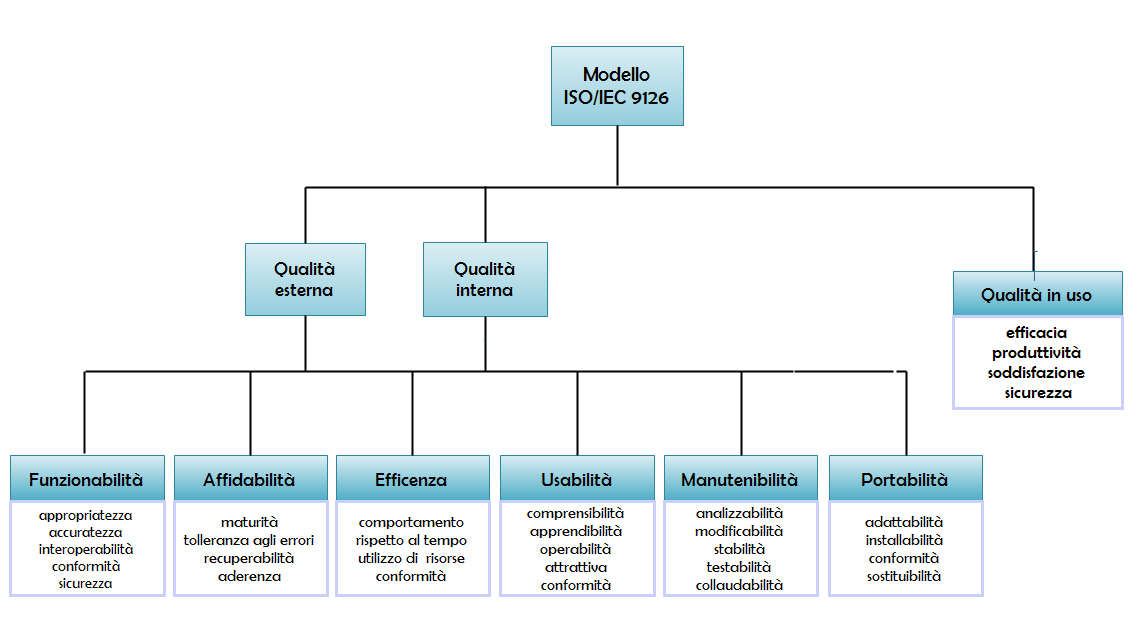
\includegraphics[width=\textwidth]{img/ISO9126.png}
		\label{fig:iso9126}
		\caption[Schema ISO 9126]{Schema ISO 9126 \protect\footnotemark}
	\end{figure}

	\footnotetext{Vedere Riferimenti Informativi in §1.5.2}
	
	\begin{figure}[H]
		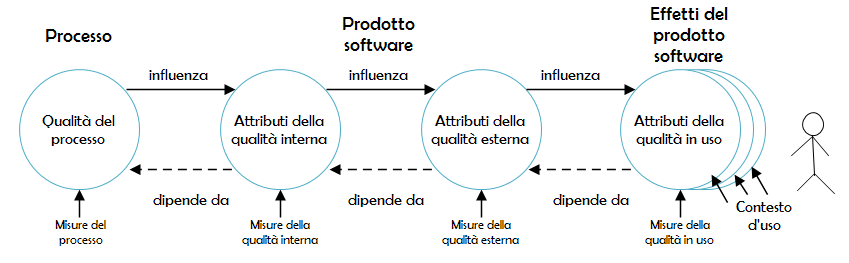
\includegraphics[width=\textwidth]{img/Ciclo_di_vita_9126.png}
		\label{fig:ciclo_di_vita}
		\caption[Ciclo di vita con l'ISO 9126]{Ciclo di vita applicando l'ISO 9126 \protect\footnotemark[1]}
	\end{figure}

	\subsection{Ciclo di Deming}
	Il ciclo di Deming è un metodo iterativo creato per migliorare la qualità dei processi e dei prodotti software. \'E un metodo che opera nell'ottica di un miglioramento continuo in termini di risultati e risorse utilizzate e al termine di ogni ciclo, l'eventuale miglioramento effettuato diventa la nuova base da cui parte l'iterazione successiva.
	
	Si distingue in quattro fasi, chiamate anche PDCA, che sono:
	
	\begin{itemize}
		\item \textbf{Plan}: pianificare i processi per ottenere i risultati attesi ed osservare dove questi possono essere migliorati;
		\item \textbf{Do}: eseguire il programma e i miglioramenti inseriti nella fase precedente;
		\item \textbf{Check}: effettuare test e controlli dell'output della fase precedente confrontandoli con gli obiettivi della fase di Plan. Dare una valutazione dei risultati per verificare se i cambiamenti attuati portano effettivamente dei miglioramenti;
		\item \textbf{Act}: le modifiche, se risultano essere delle migliorie vengono applicate al processo o al prodotto;
	\end{itemize}

	\begin{figure}[H]
		\centering
		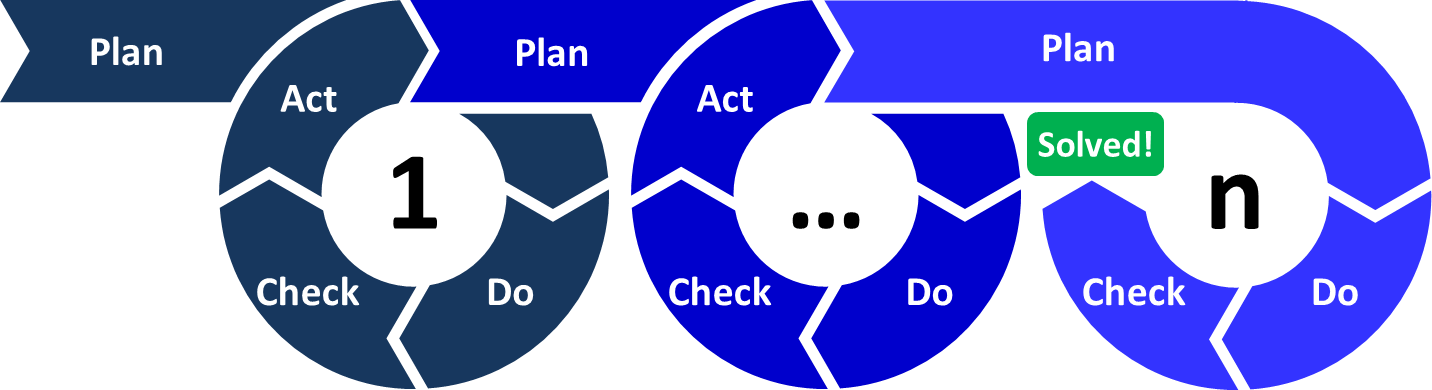
\includegraphics[width=0.65\textwidth]{img/PDCA}
		\label{fig:PDCA}
		\caption[Ciclo di Deming]{Ciclo di Deming\protect\footnotemark}
	\end{figure}

	\footnotetext{Vedere Riferimenti Informativi in §1.5.2}

	\subsection{ISO/IEC 90003:2004}
	Lo standard ISO/IEC 90003 consiste nello standard ISO 9001:2008 applicato al software. Quest'ultimo si tratta di uno standard sulla qualità dei sistemi aziendali che segue il sistema il ciclo di Deming descritto in precedenza.
	
	L'ISO/IEC 90003:2004 si suddivide in otto capitoli che sono:
	
	\begin{enumerate}
		\item Scopo
		\item Riferimenti normativi
		\item Ternimi e definizioni
		\item Sistema di gestione della qualità
		\item Gestione delle responsabilità
		\item Gestione delle risorse
		\item Realizzazione del prodotto
		\item Misurazione, analisi e miglioramento
	\end{enumerate}

	A causa delle capacità e dell'esperienza del team di sviluppo verranno presi in considerazione solo alcuni punti del quarto capitolo, in particolar modo quelli riguardante la documentazione, non potendo ancora stabilire metriche sul software.
	
	\subsubsection{Capitolo 4. dell'ISO 90003: Requisiti di Sistema e Linee guida}
	
	\begin{enumerate}
		\item \textbf{Requisiti e linee guida sull'organizzazione}
		\begin{enumerate}
			\item \textbf{Stabilire la gestione del sistema di qualità (QMS)}
			\begin{itemize}
				\item \textbf{Identificare i requisiti di cui il QMS ha bisogno}: attraverso il \PdQ~osservando i processi interni ed esterni;
				\item \textbf{Assicurarsi che ogni processo sia efficacie}: attraverso una verifica continua sui processi e prodotti;
			\end{itemize}
			\item \textbf{Documentare il proprio QMS}: riportare le relazioni tra i vari processi e come essi vengano gestiti e verificati;
			\item \textbf{Cercare di migliorare il proprio QMS}: applicando il ciclo di Deming;
			\item \textbf{Mantenere la qualità del QMS}
		\end{enumerate} 
		
		\item \textbf{Requisiti e linee guida sulla documentazione}
		\begin{enumerate}
			\item \textbf{Documentare la qualità}
			\begin{itemize}
				\item \textbf{Pianificare la documentazione del QMS}: assicurandosi che quello che verrà scritto rispecchi gli obiettivi e la gestione dei processi;
				\item \textbf{Stabilire la documentazione del QMS}: stabilendo la qualità delle diverse parti del QMS;
				\item \textbf{Mantenere la documentazione nel tempo}
			\end{itemize}
			
			\item \textbf{Controllare la qualità dei documenti}
			\begin{itemize}
				\item \textbf{Stabilire una procedura per controllare i documenti}: documentare la stessa procedura di controllo che dovrebbe contenere la fase di approvazione del documento, un suo versionamento e continuo aggiornamento;
				\item \textbf{Mantenere ed aggiornare la procedura di controllo del documento}
			\end{itemize}
		\end{enumerate}
	\end{enumerate}
